\documentclass[journal,sort]{IEEEtran}

\usepackage{lineno,hyperref}
\usepackage{bm}
\usepackage{cancel}
\usepackage{booktabs}
\usepackage{multirow}
\usepackage{array,chngpage}
\usepackage{subfigure}
\usepackage{amssymb}
\usepackage{graphicx}
\usepackage{amsmath}
\usepackage{bm}
\usepackage{diagbox}
\usepackage{cite}
\usepackage{threeparttable}
\usepackage{url}
\usepackage{setspace}
\usepackage{caption}
\DeclareMathOperator*{\argmax}{argmax}
\usepackage[linewidth=1pt]{mdframed}
\usepackage{lipsum}
\usepackage{booktabs}
\usepackage{color}
\usepackage{longtable}


\bibliographystyle{IEEEtran}

\begin{document}

\title{Adaptive and Generative Intra-frame Steganography in HEVC Video Using the Intra Block Partitioning Structure}
\author{XXXX}
	

\maketitle

\begin{abstract}
Intra-frame steganography in HEVC video is a challenge task in the field of video steganography.In this paper, steganographic characteristic of HEVC intra block partitioning structure is first analyzed. It is proved that visual quality of stego video tends to become nearly unchanged after modifying intra block partitioning structure, but the coding efficiency and security of stego video will decrease to some extent.
Based on this property, a novel steganography method based on intra block partitioning structure is proposed to embed the secret payload. In the proposed method, the secret message is not embedded into videos by modifying the cover, but is utilized to generate the cover by a generator. The cover generator can generate four different kinds of intra block partitioning structure with different depth to make full use of HEVC intra-coding structure for high-efficient video steganography.To minimize the potiential statistical detectability, an adaptive matching scheme is designed to use the appropriate generated cover for different video content.
The proposed method is examined on HD video database with different resolution and video contents,and results are further compared with previous Intra-frame steganography method to confirm the effectiveness and advantages of this method. Results also prove that compared to the traditional intra-frame cover, the intra prediction modes, the intra block partitioning structure is a more efficient and secured intra-frame hidden cover for HEVC video.


	
	
\end{abstract}	
\begin{IEEEkeywords}
		video steganography, HEVC, block partitioning structure, generative steganography
\end{IEEEkeywords}
	
\section{Introduction\label{intro}}

As an important method to ensure communication security in the network environment, Steganography has always been a key, cutting-edge research area. Steganography utilizes the characteristics of massive data exchange in the Internet, constructs a hidden channel that humans cannot detect, and transmits a large amount of secret information. This technology is both a new opportunity and a new challenge for the security communication.


One of the most challenge research task in steganography is video steganography. As a carrier of large capacity, high concealment, redundant space diversity and robustness, video has more theoretical research significance and value than image and audio steganography. Taking HEVC coded video as an example, the coding standard designed for high-definition video, the amount of data of high-definition video itself is huge, and its coding technology also brings a new coding domain steganography space, in technical complexity, algorithm security and hidden The diversity of write space is more suitable for security information steganography.

Many works have been done in both H.264/AVC and HEVC [3, 4]. Hu et al. [5] proposed a steganographic algorithm based on intra prediction mode in H.264/AVC. Yang et al. [6] have improved Hu’s method by matrix coding. Bou-chama [7] divided the intra prediction modes in H.264/AVC into four groups ac-cording to their prediction direction, the result shows a better video quality while ensuring high capacity. Zhang et al. [8] analyzed the texture of the video, and pro-posed a high security adaptive embedding algorithm using STC. Wang et al. [9] proposed intra prediction mode based method for HEVC, a mapping between an-gle difference and secret message was established to embed data. Dong et al. [10] further proposed the prediction mode steganography technology under the HEVC standard, and made a breakthrough in the capacity limitation of the previous HEVC intra prediction mode based algorithm, while also improving the security.

The contribution of  this paper including:1) a novel cover generator is proposed to 


The rest of this paper is organized as follows: In Section
2, the Steganographic characteristic of HEVC intra quadtree partition structure is described. In Section 3, the
The proposed Steganographic method for HEVC incluing the cover geneator and the mathing scheme is presented.
Section 4 gives the framework of the proposed method. Section 5 describes the experiments and results analysis for
HEVC videos. Section 5 draws the conclusion.
\section{Steganographic characteristic of Intra Block Partitioning Structure in HEVC}
In this section, the HEVC intra block partitioning structure will be first described, with which distortion analysis of visual quality, coding efficiency and security in HEVC intra steganographic algorithm can be thoroughly introduced next.
\subsection{Intra Block Partitioning Structure in HEVC }
As in all prior ITU-T and ISO/IEC JTC 1 video coding
standards since H.261, the HEVC design follows the
classic block-based hybrid video coding approach. The basic source-coding algorithm is a hybrid
of interpicture prediction to exploit temporal statistical dependences,
intrapicture prediction to exploit spatial statistical
dependences, and transform coding of the prediction residual
signals to further exploit spatial statistical dependences[].Compared with the previous coding standards, HEVC proposes and adopts some new coding technologies based on  the classic block-based hybrid coding approach. With the introduction of these new technologies, the coding efficiency of HEVC has been greatly improved. The intra quadtree block partitioning structure is one of these key technologies.


The HEVC standard has adopted a highly flexible and efficient block partitioning structure. Frames are splited into an integer multiple of CTU, which is an analogous term to the macroblock in H.264/AVC. A CTU consists of one luminance CTB and two chrominance CTB.The terms coding
tree block (CTB) is defined to specify the 2-D sample array of one color component associated with the CTU. In the CTU, a quadtree is established. Let CTU size be 2N$\times$2N where N is one of the values of 32, 16, or 8. The CTU can be further recursively split into four smaller units of equal sizes of N$\times$N, which are nodes of the quadtree. If the
units are leaf nodes of the quadtree, the units become coding units (CUs).


HEVC utilizes CU as a unit to specify which prediction
scheme is used for intra and inter predictions. 
Although use of a quadtree structure in video compression is not a new concept, the coding tree approach in HEVC can bring additional coding efficiency benefits by incorporating PU and TU quadtree concepts for video compression.

Leaf nodes of a tree can be merged or combined [22] in a general quadtree structured video coding scheme. After the final quadtree is formed, motion information is transmitted at the leaf nodes of the tree. L-shaped or rectangular-shaped motion partition is possible through merging and combination of nodes. However, in order to make such shapes, the merge process should be followed using smaller blocks after further splitting is occurred. in the HEVC block partitioning structure, such cases are taken care of by the PU [15]. Instead of splitting one depth more for merging and combination, predefined partition modes such as PART\_2N×2N, PART\_2N×N, and PART\_N×2N are tested and the optimal partition mode is selected at the leaf nodes of the tree. It is worthwhile mentioning that PUs still can share motion information through merging mode in HEVC. Although a general quadtree structure without PU concept was investigated by removing the symmetric rectangular partition modes (PART\_2N×N and PART\_N×2N) from the syntax and replaced by corresponding merge flags [23], both coding efficiency and complexity was proved inferior to the current design.

Another difference is the transform tree. Even though variable block size transforms were used for quadtree structured motion compensation, their usage was rather restricted. for example, transform size was strictly combined with motion compensation block size. Even though multiple transform size could be utilized, it was usual to use same size transform in a motion compensated block. in HEVC, the motion compensated residual can be transformed with a quadtree structure, and the actual transform is performed at leaf nodes. Since the transform tree is rooted from the leaf nodes of coding tree, this creates a nested quadtree. This kind of nested quadtree exists since the transform tree is started from the CU regardless of partition modes, i.e., PU shapes [16]. This is a way to construct a nested quadtree even though we have PU concepts that differ from a general quadtree structure.

Another noticeable aspect is the full utilization of depth information for entropy coding. for example, entropy coding of HEVC is highly reliant on the depth information of quadtree. for syntax elements such as inter\_pred\_idc, split\_transform\_flag, cbf\_luma, cbf\_cb and cbf\_cr, depth dependent context derivation is heavily used for coding efficiency. It has been demonstrated that this can break the dependency with neighboring blocks with less line buffer requirement in hardware implementations because information of above CTU does not need to be stored.

\begin{figure}[htbp!]
	\centering
	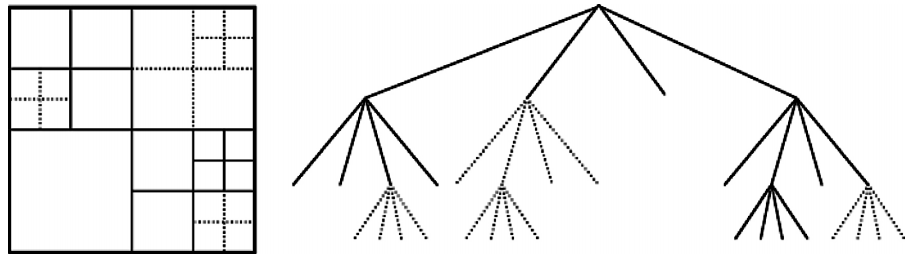
\includegraphics[width=0.5\textwidth]{1.png}
	\caption{HEVC intra partitioning structure}
	\label{HEVC-part}
\end{figure}


The PB size, which is the block size at which the intra prediction mode is estab-lished is the same as the CB size except for the smallest CB size (usually 8×8) is allowed in the bitstream. For the latter case, a flag is present that indicates whether the CB is split into four PB quadrants, each PB with their own intra prediction mode. The actual region size at which the intra prediction operates depends on the residual coding partitioning. 
For residual coding, a CB can be recursively partitioned into Transform Blocks (TBs). The partitioning is signaled by a residual quadtree. Intra prediction operates based on the TB size, and previously decoded boundary samples from spatially neighboring TBs are used to form the prediction signal. Directional prediction with 33 different directional orientations is defined for (square) TB sizes from 4×4 to 32×32. 

\subsection{Distortion Analysis on visual quality}
According to the HEVC intra coding scheme, this subsection will present the analysis of visual quality degradation caused by HEVC steganography, in order to illustrate the reason why large-sized PBs can be modified without introducing significant visual distortion.
Spatial-domain intra prediction has previously been successfully used in H.264/ AVC. The intra prediction of HEVC operates similarly in the spatial domain, but is extended significantly—compared to the eight prediction directions of H.264/AVC, HEVC supports a total of 33 angular prediction directions with DC and Planar mode.

\subsection{Distortion Analysis on coding efficiency}
\subsection{Distortion Analysis on Security}
\section{The proposed Steganographic method for HEVC}

\subsection{The cover generator}

\subsection{The adaptive matching scheme}
\section{Framework}



\section{Experimental results}
\section{conclusion}




	
	
	
	
	
	
	
\end{document}